Yet another classic Q-switching question.
If you keep your head cool then you should be able to bag at least 20 marks from this question.
\begin{parts}
	\part \textit{Mostly copypasta from Q1 2019.}
	
	Q-switching is a technique by which the quality factor of a laser cavity is periodically varied to intentionally build up population inversion $N^*$ beyond the equilibrium value, thus producing a laser output with \textit{large peak intensity} and \textit{short pulse length}.
	
	Q-switching may be achieved by employing a saturable absorber at the output coupler.
	As the absorption of the absorber varies with the intensity $I$, it is able to suppress lasing until saturation, thereby achieving Q-switching without active clock source.
	
	Sketch of the cavity setup:
	\begin{figure}[H]
		\centering
		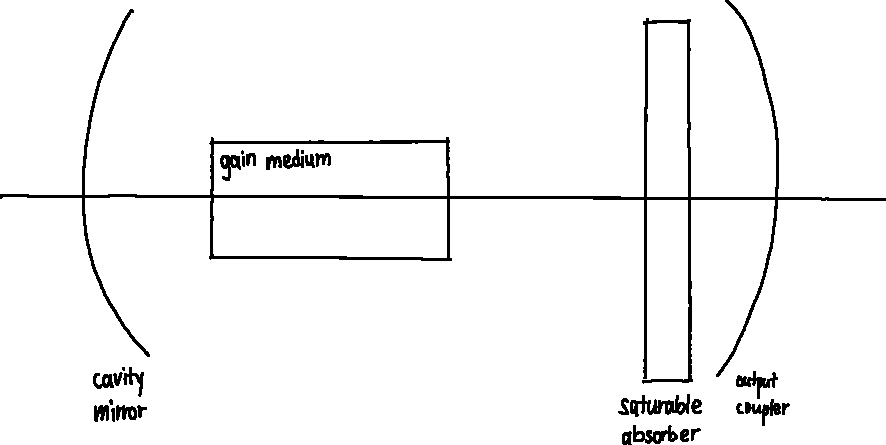
\includegraphics[width=.8\linewidth]{q1-cavity}
	\end{figure}
	
	\part Usual bookwork, from the rate equations we immediately see that the contribution in cavity photon density due to lasing is given by $N^* \sigma_{21} I / \hbar\omega$.
	
	We also know that intensity $I = n \hbar\omega c$, together with the careful consideration that the lasing medium takes up only a fraction $f_c$ of the cavity:
	\begin{equation}
		\deri{n_\textnormal{lasing}}{t} = f_c N^* \sigma_{21} nc
		\label{eqn:q1-photon-density-lasing}
	\end{equation}
	
	Taking cavity loss into account then yields the total rate of change in cavity photon density:
	\begin{align}
		\deri{n}{t} &= \deri{n_\textnormal{lasing}}{t} - \frac{n}{\tau_c} \notag \\
		&= \rbracket{f_c N^* \sigma_{21} c \tau_c - 1} \frac{n}{\tau_c} \notag \\
		&= \rbracket{\frac{N^*}{N^*_\textnormal{th}} - 1} \frac{n}{\tau_c}
		\label{eqn:q1-dn-dt}
	\end{align}
	where $\tau_c$ is the cavity lifetime, and $N^*_\textnormal{th} = \rbracket{f_c \sigma_{21} c \tau_c}^{-1}$ is the threshold population inversion which signifies the minimum population inversion required for the cavity photon density to grow.
	
	\part Another bookwork.
	We consider the simplified rate equations by ignoring the pump and spontaneous terms:
	\begin{gather}
		\deri{N_2}{t} = - \frac{N^*}{N^*_\textnormal{th}} \, \frac{n}{f_c \tau_c} \label{eqn:q1-dn2-dt} \\
		\deri{N_1}{t} = \frac{N^*}{N^*_\textnormal{th}} \, \frac{n}{f_c \tau_c}
		\label{eqn:q1-dn1-dt}
	\end{gather}
	
	We then have population inversion $N^* = N_2 - g_2 / g_1 N_1$, so
	\begin{align}
		\deri{N^*}{t} &= - \underbracket{\rbracket{1 + \frac{g_2}{g_1}}}_{\beta} \frac{N^*}{N^*_\textnormal{th}} \, \frac{n}{f_c \tau_c}
		\label{eqn:q1-dN*-dt} \\
		&= -\beta \sigma_{21} c N^* n \notag
	\end{align}
	
	To find the output energy, we first consider the power output $P$ of the cavity:
	\begin{align}
		P &= \rbracket{\textnormal{rate of photon ejection}} \times \hbar\omega  \notag \\
		&= \frac{nV_c \hbar\omega}{\tau_c}
		\label{eqn:q1-output-power}
	\end{align}
	where $V_c$ is the cavity volume.
	
	Then we integrate \eqref{eqn:q1-output-power}, noting the usual trick of dummy substitution\footnote{Also a potential footgun here: $N^*_f$ is not the same as $N^*_\textnormal{th}$! The author had the misfortune of stepping on this trap and lost a couple of marks\dots}:
	\begin{align*}
		E &= \defint{-\infty}{\infty}{P}{t} \\
		&= \int_{-\infty}^{\infty} \inftsml{t} \, \hbar\omega V_c \frac{n}{\tau_c} \\
		&= \int_{-\infty}^{\infty} \inftsml{t} \, \hbar\omega V_c \frac{N^*}{N^*_\textnormal{th}} \frac{n}{\tau_c} \\
		&= - \int_{N^*_i}^{N^*_f} \inftsml{N^*} \, \hbar\omega V_c \frac{f_c}{\beta} \\
		&= \rbracket{N^*_i - N^*_f} \hbar\omega V_c \frac{f_c}{\beta} \\
		&= \underbracket{\frac{1-N^*_f/N^*_i}{\beta}}_{\eta} V_g \hbar\omega
	\end{align*}
	where $\eta$ is the energy utilisation factor -- it encodes how efficient a laser system is in extracting energy from population inversion.
	
	Observe that the case with 3-level laser corresponds to severe bottlenecking where $\beta > 1$, making it less efficient than an otherwise similar 4-level system where $\beta = 1$.
	
	\part Yet another bookwork.
	Overpumping ratio $r$ is defined as
	\begin{equation}
		r = \frac{N^*_i}{N^*_\textnormal{th}}
	\end{equation}
	which encodes how far away the initial population inversion before pulse is from the threshold value.
	
	Following the sketch below, we see that higher $r$ will lead to a more intense and shorter pulse.
	\begin{figure}[H]
		\centering
		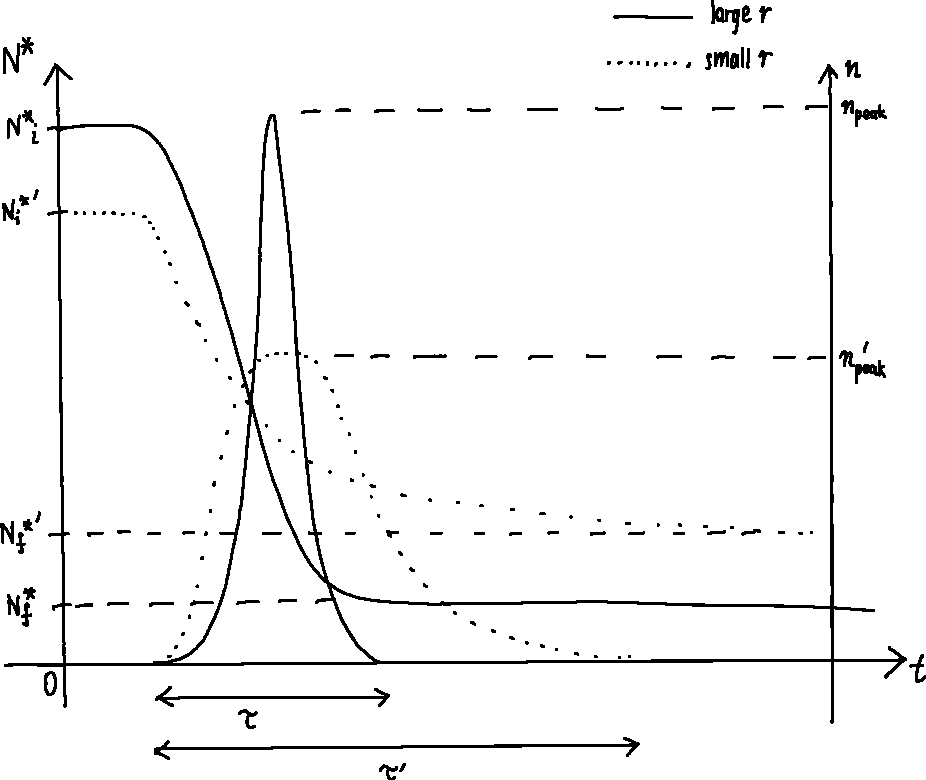
\includegraphics[width=.9\linewidth]{q1-pulse-sketch}
	\end{figure}
	
	Now to relate between $r$ and $E$, we need to first eliminate $N^*_f$ -- this can be done by dividing \eqref{eqn:q1-dn-dt} with \eqref{eqn:q1-dN*-dt} to get:
	\begin{equation}
		\deri{n}{N^*} = -\frac{f_c}{\beta} \frac{N^*/N^*_\textnormal{th} - 1}{N^*/N^*_\textnormal{th}}
		\label{eqn:q1-dn-dN*}
	\end{equation}
	
	Solving \eqref{eqn:q1-dn-dN*} then gives:
	\begin{gather}
		\defint{n(t=0)}{n(t)}{}{n} = -\int_{N^*_i}^{N^* (t)} \inftsml{N^*} \, \frac{f_c}{\beta} \rbracket{1 - \frac{N^*_\textnormal{th}}{N^*}} \notag \\
		n(t) - 0 = -\frac{f_c}{\beta} \sbracket{\rbracket{N^* (t) - N^*_i} - N^*_\textnormal{th} \rbracket{\ln N^* (t) - \ln N^*_i}} \notag \\
		\Rightarrow n(t) = \frac{f_c}{\beta} \sbracket{N^*_\textnormal{th} \ln\rbracket{\frac{N^* (t)}{N^*_i}} - \rbracket{N^*(t) - N^*_i}}
		\label{eqn:q1-n(t)}
	\end{gather}
	
	Substituting $n(t\rightarrow\infty) = 0$ and $N^* (t\rightarrow\infty) = N^*_f$ into \eqref{eqn:q1-n(t)} then gives:
	\begin{gather*}
		N^*_f - N^*_i = N^*_\textnormal{th} \ln\rbracket{\frac{N^*_f}{N^*_i}} \\
		\Rightarrow \underbracket{1 - \frac{N^*_f}{N^*_i}}_{\beta\eta} = -\frac{1}{r} \ln\underbracket{\rbracket{\frac{N^*_f}{N^*_i}}}_{1 - \beta\eta}
	\end{gather*}
	
	Hence for the energy output to reach $\SI{95}{\percent}$ of its maximum, we need:
	\begin{gather*}
		\beta\eta = \SI{95}{\percent} \\
		\Rightarrow 0.95 = -\frac{1}{r} \ln \rbracket{1 - 0.95} \\
		\Rightarrow r = 3.15
	\end{gather*}
\end{parts}